\stchapter{chap:chapter01}{Web Components}

Web Components is a new set of standards that we can use to create complex UI
widgets and application pieces. One platform for creating Web Components is
Polymer, developed by Google.

A Web Component contains elements that contain templates, styles, and logic,
all encapsulated in that component. They have four specifications which are:

\begin{itemize}
    \item Templates
    \item Shadow Dom
    \item Custom Elements
    \item HTML Imports
\end{itemize}

\stsection{sec:firstSection}{Templates}{}{}\label{sec:01--templates}


Templates are fragments of HTML for which the content is not loaded, until you get its content using Javascript without
using AJAX, such content can be saved inside the \texttt{<template>} and retrieved later.

\lstinputlisting{./code/src/chapter01/components/superman/superman.html}

The element is pulled doing something as follows:

\lstinputlisting{./code/src/chapter01/components/superman/superman.js}

Of course a component wouldn't be complete with some styling attached to it:

\lstinputlisting{./code/src/chapter01/components/superman/superman.scss}

To pull this we are using webpack. The original image I'm using is 1361x561, but we modify that
property on load to get an the following:

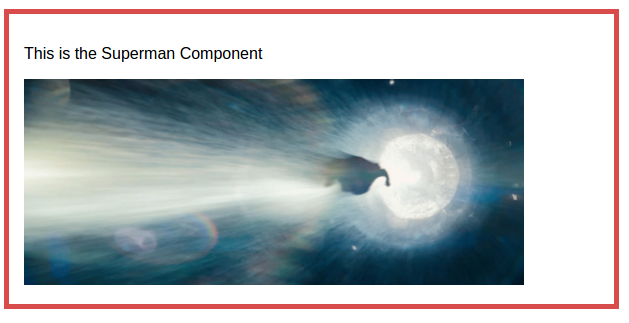
\includegraphics[width=0.5\linewidth]{./src/images/screenshot--superman.png}

\stsection{sec:01--adding-templates}{Ways of adding templates}{}{}
\label{sec:01--adding-templates}

There are essentially four ways of adding templates

\stsubsection{ssec:01--hidden-elements}{Hidden elements}{}{}
\label{ssec:01--hidden-elements}

Copy/Pasting it the hardcore way.

\begin{lstlisting}
<div hidden data-template="superman">
    <div>
        <p>SuperMan Template</p>
        <img src="assets/img/superman.png" class="animated_superman"/>
    </div>
</div>
\end{lstlisting}

\huge{CONS:} The browser loads unnecessary markup, and when pasted it wont load the images, video, audio.

\stsubsection{ssec:01--pull-content}{Ajax all the things}{}{}
\label{ssec:01--pull-content}

\huge{CONS:} Unnecessary noise. Pulling it by Ajax is downright a bad implementation.
Somebody could inject bad code using Cross Site Script.

\stsubsection{ssec:01--x-template}{Use a local script template}{}{}
\label{ssec:01--x-template}

\begin{lstlisting}
<script data-template="superman" type="x-template">
    <div>
        <p>SuperMan Template</p>
        <img src="assets/img/superman.png" class="animated_superman"/>
    </div>
</script>
\end{lstlisting}

\huge{CONS:} Unnecessary noise when working with strings.

\stsubsection{ssec:01--compiled-templates}{Compiled templates}{}{}
\label{ssec:01--compiled-templates}

A Template engine handles it and you work with the string.

\huge{CONS:} Unneceessary noise when working with strings.

\stsection{sec:01--shadow-dom}{Shadow DOM}{}{}
\label{sec:01--shadow-dom}

The \texttt{audio}, \texttt{video}, \texttt{a}, \texttt{input} are de best examples to describe the
functionality provided by the Shaodw DOM. Those elements are web components, and we don't see the
internal implementation of these tags.